%!TEX root = ../thesis.tex

\graphicspath{{assets/chapter_1/}}

\chapter{Introduction}\label{ch:introduction}
% \chapter{Summary of research problems and contribution}

\begin{section}{Motivation}
	The quest for better wireless connectivity has been long-standing since Marconi's illuminating radio in 1895.
	Great successes have been made at the transmitter and receiver sides over the past century, and the communications society is unprecedentedly close to the Shannon limit \cite{Shannon1948}.
	By 2025, global mobile data traffic is expected to reach {607} exabytes per year \cite{Tariq2020} while the number of connected devices may exceed {75} billion \cite{Georgiev2024}.
	At the same time, wireless applications are also evolving in various forms to address world-changing incidents like COVID-19, climate change, geopolitical tensions, and \gls{ai} revolution.
	An initial attempt was made in 5G where the network prioritizes among high-throughput, ubiquitous-coverage, high-reliability, low-latency, massive-connectivity, and energy-efficient services \cite{Shafi2017}.
	However, the desire of human and machine for better communication shows no signs of slowing down.
	Emerging applications such as smart cities, autonomous driving, telemedicine, extended reality, federated learning, and generative intelligence are calling for a stronger and smarter wireless infrastructure.
	It is envisioned that 6G will be designed to meet the following requirements \cite{Tataria2021,Alsabah2021,Jiang2021}:
	\begin{itemize}
		\item \emph{Throughput:} The network would be able to provide a peak data rate of 1 Tbps and an average data rate of 100 Gbps per user.
		\item \emph{Latency:} Sub-millisecond end-to-end latency would be achieved for low-latency applications like autonomous driving and remote surgery.
		\item \emph{Reliability:} A success rate of 99.9999\% would be guaranteed for ultra-reliable applications like industrial automation and cooperative robotics.
		\item \emph{Connectivity:} The number of connected devices per kilometer square would be increased to 10 million for supporting \gls{ioe}.
		\item \emph{Mobility:} Commercial airlines with a maximal velocity of 1000 km/h would be the target application scenario.
		\item \emph{Energy efficiency:} Power consumption has been a major criticism for 5G. It is expected that energy per bit would be reduced by over 90\% in 6G to reduce carbon footprints.
		\item \emph{Positioning accuracy:} Thanks to THz base stations, a 3D positioning accuracy of centimeter level may be achieved for indoor and outdoor environments.
		\item \emph{Coverage:} Poor coverage has been another bottleneck for 5G. A terrestrial-satellite-aerial integrated network would provide a ubiquitous and uniform coverage for urban, rural, and remote areas.
		\item \emph{Security and privacy:} Physical-layer security can be improved with narrower beams at higher frequencies and destructive scattering at the environment. Privacy can be enhanced with federated learning and homomorphic encryption.
		% \item \emph{Superintelligent:} The network may integrate human, machine, environment, and \gls{ai} into a superintelligent system that can sense, communicate, and act in a coordinated manner.
	\end{itemize}

	Beyond the statistical requirements above, the next-generation wireless network is desired to integrate human, machine, environment, and \gls{ai} seamlessly for a harmonic ecosphere.
	This paradigm shift from \emph{connectivity} to \emph{intelligence} is fueled by the latest advances in machine learning (theory) and programmable metamaterials (hardware).
	The former enables the network to understand the environment while the latter evolves the environment from a chaotic medium to a conscious agent that can serve on demand.
	Together, they form a symbiotic relationship with the potential to revolutionize how the world energize, sense, communicate, and interact.

	One promising candidate within this 6G vision is \gls{ris}, a programmable metasurface that recycles and redistributes the electromagnetic waves in the air for improved wireless performance.
	It could be incorporated into the transmitter and receiver for \emph{beamforming}, employed as a free-rider information source for \emph{modulation}, or simply placed in space as a standalone device for \emph{channel shaping}.
	These applications have distinctive requirements and trade-offs, but the operation principles are the same and those roles are not mutually exclusive.
	Imagine a future where everything can be ``smartened'' by coating with a metamaterial layer and attaching a microcontroller tag.
	Only a few active radiating sources (like the sun) are needed, while most objects (like the universe) can exploit the surrounding waves to energize themselves, sense the environment, communicate with others, and help those in need when idle.
	This vision motivates three research questions to be addressed in this thesis:
	\begin{itemize}
		\item \emph{How does \gls{ris} impact different wireless applications such as communication and far-field power transfer?}
		\item \emph{Is it possible to integrate \gls{ris} with \gls{bc} into a versatile tool that blurs the boundary between the network and environment?}
		\item \emph{What is the ultimate limit of channel reshaping through passive \gls{ris} and what are the implications on transceiver designs?}
	\end{itemize}

	Before delving into these questions, we first provide a short overview of \gls{ris} and introduce some potential applications.
	A detailed literature review and technical discussion on \gls{ris} and other topics will be reserved for Chapter \ref{ch:background}.
\end{section}

\begin{section}{Overview on \glsfmtfull{ris}}\label{sc:ris_overview}

	% Compared with traditional multi-antenna techniques, \gls{ris} has the potential to achieve a similar performance using fewer active components, lower power consumption, and lower hardware complexity.
	% It also features no \gls{rf} chains, no symbol dependency, minimum signal processing, negligible additional noise, and can be deployed in various forms (e.g., walls, windows, ceilings, tables) to provide seamless coverage and powerful customization for indoor and outdoor environments.
	% These unique characteristics make \gls{ris} a ubiquitous and cost-effective solution for future wireless communication, sensing, and power transfer systems.

	% and may be evolved into a versatile tool, which blurs the boundary between the network and environment.
	% This vision motivates us to explore the fundamental limits of \gls{ris} and integrate it with state-of-the-art wireless technologies.

	% Despite the great possibilities, the prototyping of \gls{ris} is still in its infancy and no commercial product has been released by the first quarter of 2024.
	% The transition from theory to practice is hindered by many challenges, such as channel acquisition, response resolution, out-of-band response mitigation, placement optimization, and integration with existing systems.
	% Most importantly, a comprehensive understanding of its potential is still missing and the precise role it shall play in 6G remains ambiguous.

	\begin{subsection}{Concept}
		\gls{ris} is commonly known as a planar surface involving numerous wave scattering elements (a.k.a. unit cells, reflective patches), whose amplitude and phase responses can be engineered in real-time to achieve a desired radiation pattern.
		It behaves like a delicate \gls{rf} mirror with adjustable curvature and orientation, which allows the incident signals to be focused and redirected in a particular direction.
		As shown in Fig. \ref{fg:ris_architecture}, its typical architecture consists of three stacked layers and a controller \cite{Wu2020}.
		The top layer is a two-dimensional array of scattering elements printed on a dielectric substrate.
		The elements directly interact with the impinging waves, which are usually fabricated from metamaterial or patch/dipole antennas with sub-wavelength dimension and spacing.
		The middle layer is a copper ground plate that provides voltage reference and avoids signal leakage.
		The bottom later is a circuit board that associate each element with adjustable components, such as varactor and \gls{pin} diodes \cite{Dai2020}.
		It also hosts a \gls{fpga} controller that controls the circuit and coordinate with transceivers in the network.
		By adjusting the scatter response of all elements, the \gls{ris} can effectively manipulate the wavefront for a constructive or destructive superposition and thus improve the ambient wireless environment.
		\begin{figure}
			\centering
			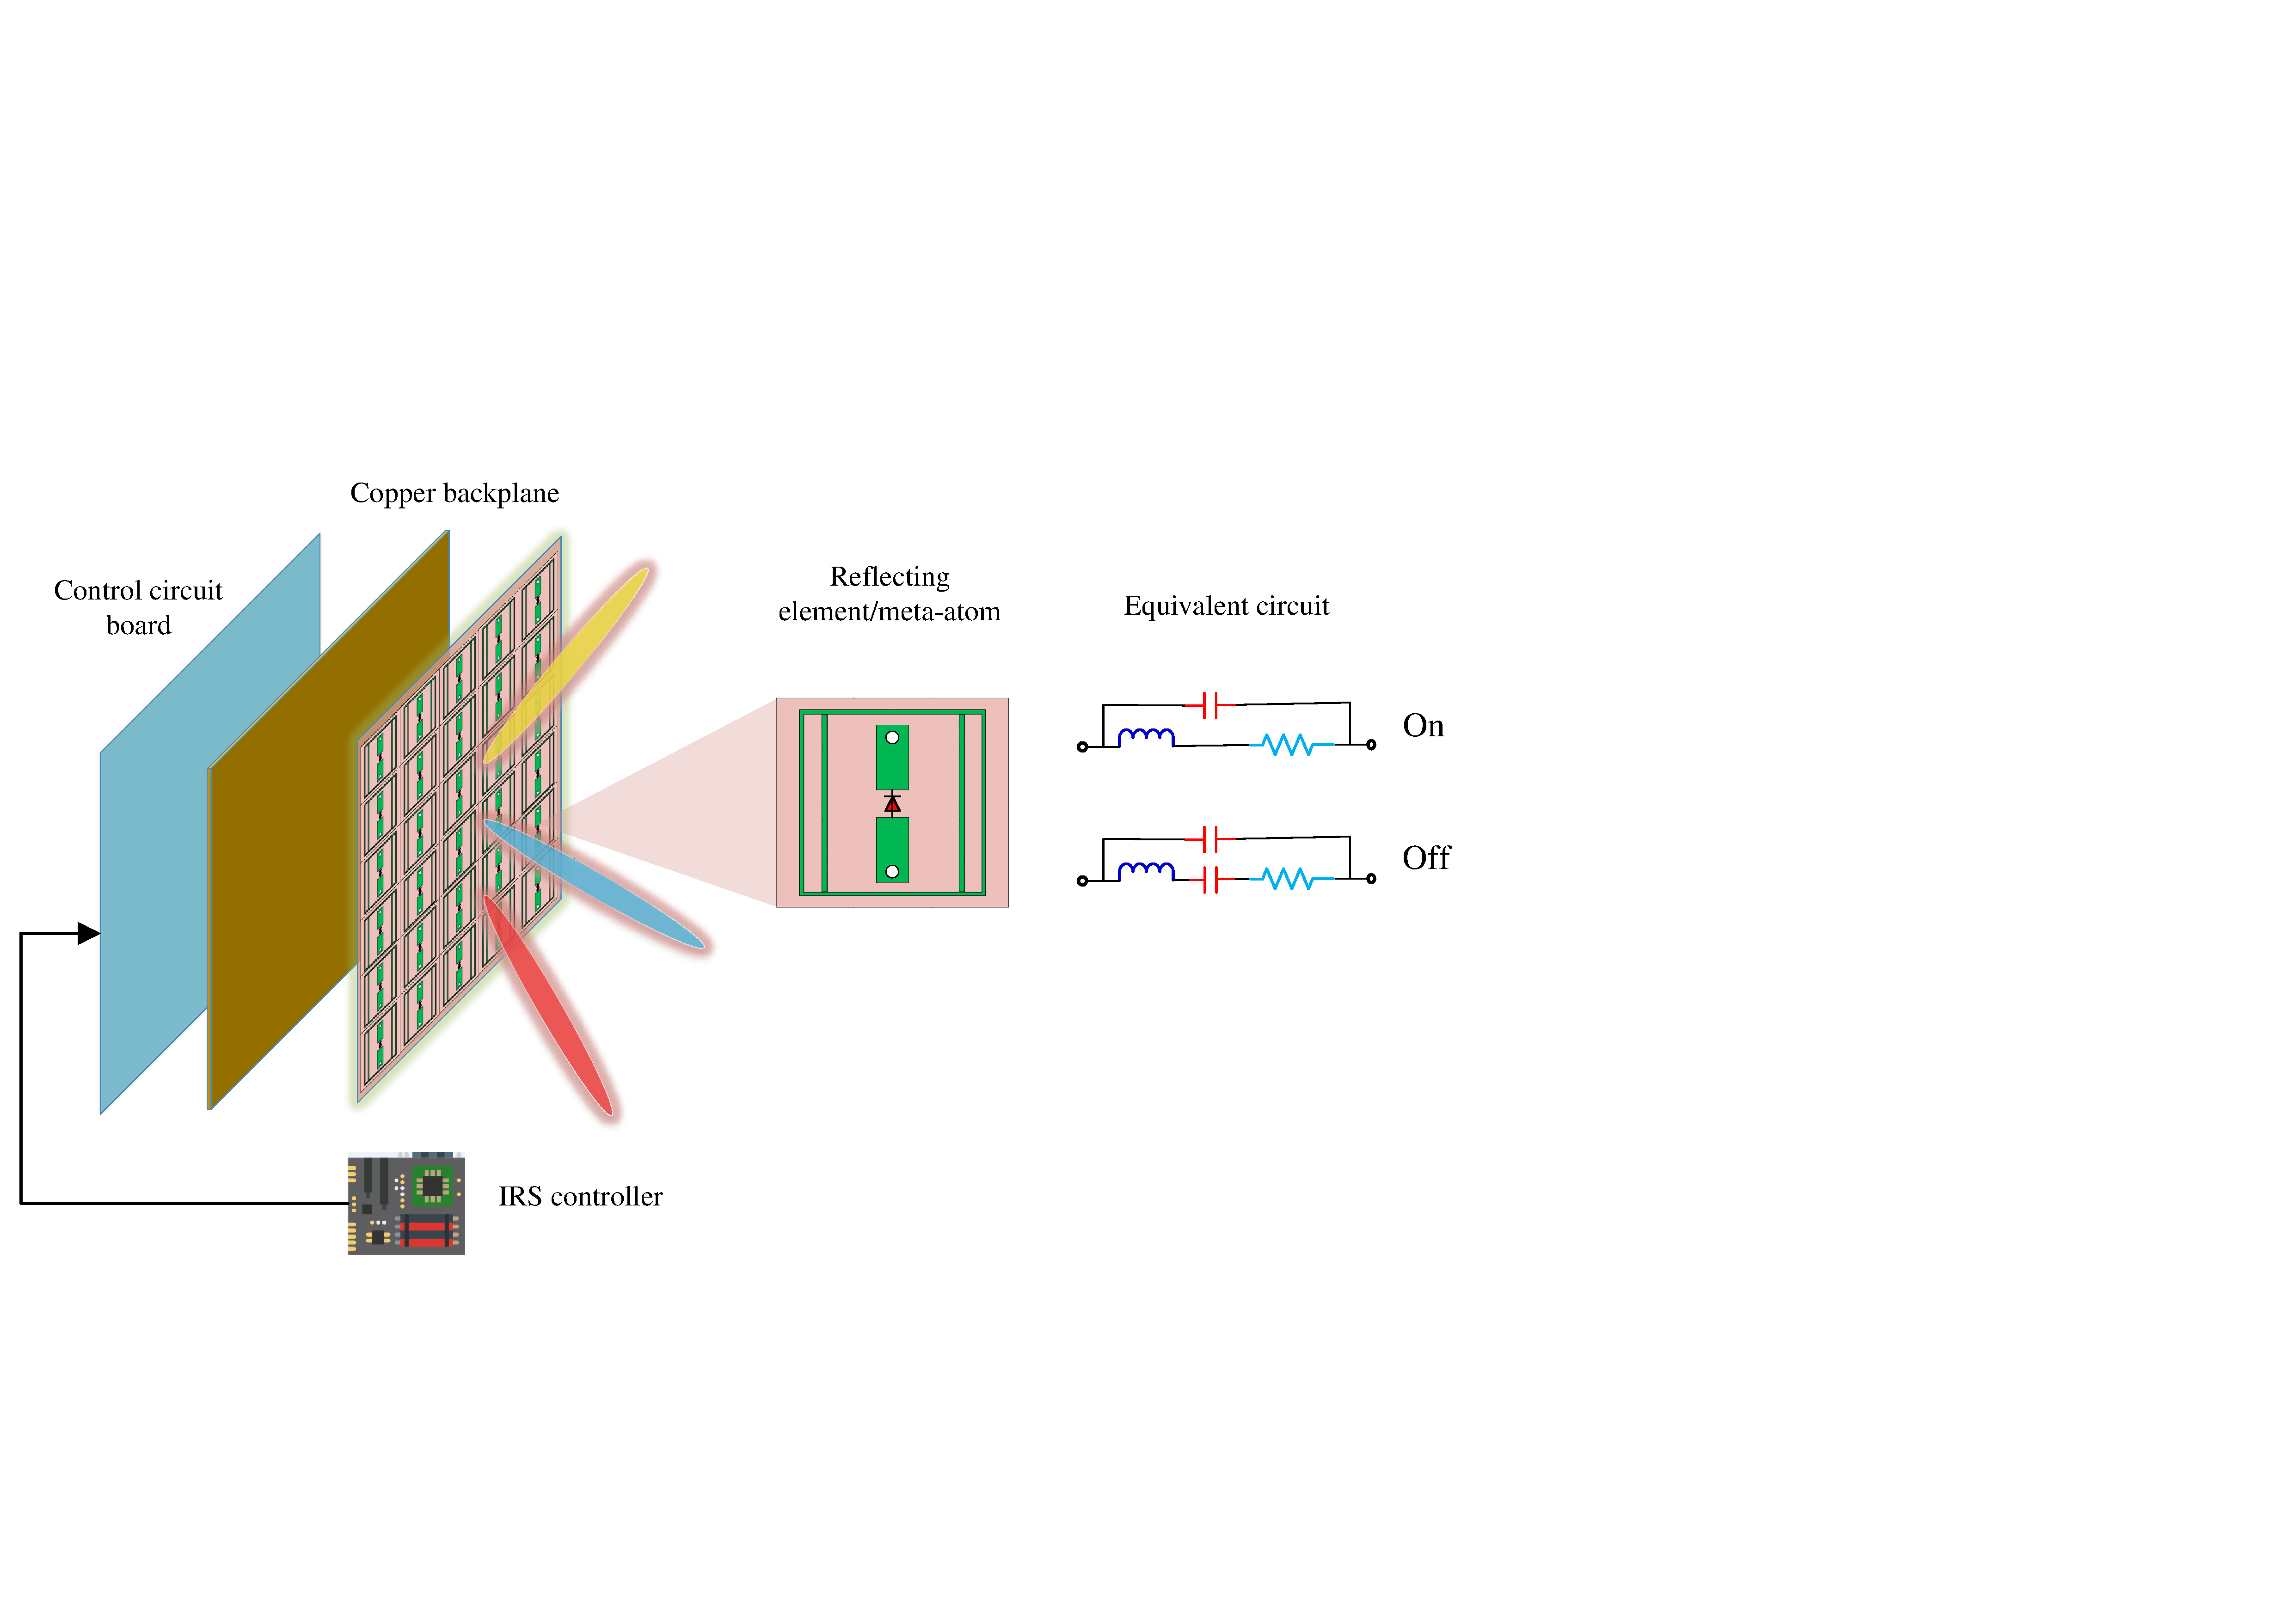
\includegraphics[width=0.9\textwidth]{ris_architecture.pdf}
			\caption{A typical architecture of \gls{ris}. The figure is modified from \cite{Wu2020}.}
			\label{fg:ris_architecture}
		\end{figure}
	\end{subsection}

	\begin{subsection}{Characteristics}
		The key characteristics of \gls{ris} are summarized as follows:
		\begin{itemize}
			\item \emph{Passive and environmental-friendly:} \gls{ris} reflects the incident waves in a passive manner and does not require dedicated \gls{rf} chains.\footnote{The controller may be implemented with low-power components and powered by ambient energy.} This is different from \gls{af} relays that require power-hungry oscillators and introduces additional thermal noise.
			\item \emph{Flexible:} It provides a software configurable environment that can be adapted for different applications and scenarios. This is different from conventional reflectarray \cite{Nayeri2018} and frequency selective surfaces \cite{Anwar2018} with predefined radiation patterns and frequency response.
			\item \emph{Full-duplex and universal:} This physical-layer solution can simultaneously support communication, sensing, and power transfer without self-interference. Thanks to channel reciprocity, the optimal configuration for downlink and uplink coincide with each other \cite{Wu2021}. This is different from \gls{df} relays that are designed for a specific communication link and suffers from packet delays.
			\item \emph{Low-cost and conformal:} It can be manufactured from low-cost materials and deployed in various forms (e.g., walls, windows, ceilings, tables) to provide seamless coverage and powerful customization for indoor and outdoor environments. This is different from conventional multi-antenna systems that features complex hardware and bulky structures.
		\end{itemize}
	\end{subsection}

	\begin{subsection}{Applications}\label{sc:ris_applications}
		The channel manipulation capability of \gls{ris} unlocks a wide range of unprecedented applications, such as signal enhancement \cite{Wu2019}, interference suppression \cite{Jiang2022}, blockage bypassing \cite{Ghatak2021}, coverage extension \cite{Zeng2021}, and security control \cite{Almohamad2020}.
		It also has the potential to convey additional information \cite{Ye2022}, compensate for the Doppler effect \cite{Basar2021}, transform frequency-selective channels into frequency-flat \cite{Arslan2022}, improve the spatial diversity for multi-antenna systems \cite{Ozdogan2020a}, and create artificial time diversity for multi-user orthogonal \cite{Yang2019} and non-orthogonal \cite{Chen2023} multiple accesses.

		Those fancy characteristics and applications of \gls{ris} have also attracted significant attention from the industry.
		The first public testing attempt was made in 2018 by NTT Docomo and Metawave, which demonstrated a metasurface reflectarray in the FR2 band of 5G can boost a downlink data rate from \qty{60}{Mbps} to \qty{560}{Mbps} \cite{Liu2022b}.
		Later in 2020, NTT Docomo developed a transparent dynamic \gls{ris} that can allows 28GHz signals to reflect or pass through with negligible power loss.
		A regional ``\gls{ris} alliance'' was formed in 2021 by Chinese companies and institutes including ZTE, China Mobile, and CAICT, which soon released a white paper \cite{Rista2023} to promote the technology and standardization.
		In December 2022, ITU-R drafted a recommendation report for IMT-2030 (6G) \cite{Itu2022} that marks \gls{ris} as a key technology to enhance the radio interface for multiple physical dimension transmission.
		These developments showcase the rapid progress of \gls{ris} from theoretical concept to practical implementation, paving the way for its integration into the next-generation network.
	\end{subsection}
\end{section}

\begin{section}{Outline and Contributions}
	The thesis is outlined as follows:
	\begin{itemize}
		\item Chapter \ref{ch:introduction} provides an overview of the thesis. It introduces the motivation and objectives, discusses the characteristics and applications of \gls{ris}, and summarizes the topics and contributions of each research chapter. A list of publications is also provided.
		\item Chapter \ref{ch:background} provides the necessary background knowledge for the subsequent chapters, including the fundamental principles, hardware implementation, signal and system models, performance metrics, and design challenges for \gls{ris}, \gls{wpt}, \gls{swipt}, \gls{bc}, and \gls{mimo} systems. It also reviews the state-of-the-art research in relevant topics and raise critical questions to be addressed in the following chapters.
		\item Chapter \ref{ch:ris_aided_swipt} investigate the impact of \gls{ris} on wireless information and power transfer. The key contributions include:
		\begin{itemize}
			\item Introduce \gls{ris} to a multi-antenna multi-carrier \gls{swipt} system with different receiver architectures;
			\item Consider joint waveform and beamforming design for the proposed system under a practical energy harvester model;
			\item Characterize the \gls{r-e} performance trade-off by maximizing harvested energy subject to different communication rate constraints;
			\item Propose local-optimal and low-complexity algorithms and evaluate their narrow and wideband performance through numerical simulations;
			\item Discuss the array gain for communication and the scaling order for power transfer in terms of the number of transmit antennas and \gls{ris} elements.
		\end{itemize}
		\item Chapter \ref{ch:riscatter} develops a novel scatter protocol that integrates beamforming and modulation. The key contributions include:
		\begin{itemize}
			\item Provide an in-depth comparison of \gls{ris} with state-of-the-art \gls{bc} technologies and discuss the key properties of active and passive transmissions coexisting systems;
			\item Unify \gls{ris} and \gls{bc} as one battery-free cognitive radio called RIScatter, where dispersed or co-located scatter nodes ride over an active primary link to modulate their own information and engineering the legacy channel simultaneously;
			\item Integrate backscatter modulation and passive beamforming seamlessly into the input distribution design that allows arbitrary trade-off in between;
			\item Propose a low-complexity cooperative receiver that sequentially decodes both coexisting links and exploits backscatter detection as part of channel training;
			\item Characterize the achievable primary-backscatter rate region over different designs of input distribution at the scatter nodes, active beamforming at the \gls{ap}, and energy detector at the receiver;
			\item Discuss the impact of practical factors such as the number of scatter nodes and states, transmit antenna size, backscatter symbol duration, and \gls{snr} on the system performance.
		\end{itemize}
		\item Chapter \ref{ch:channel_shaping} explores the ultimate channel shaping capabilities of \gls{ris} in \gls{mimo} systems. The key contributions include:
		\begin{itemize}
			\item Quantify the capability of a passive \gls{ris} to reshape the \gls{mimo} \gls{pc} in terms of singular values via analytical bounds and numerical optimization;
			\item Focus on a general \gls{bd}-\gls{ris} architecture featuring element-wise connections and demonstrate its superior signal processing performance (subspace alignment and subchannel rearrangement) over the widely-adopted diagonal model;
			\item Propose an efficient \gls{rcg} algorithm for general \gls{bd}-\gls{ris} optimization and provide low-complexity solutions for quadratic problems;
			\item Characterize the Pareto frontiers of channel singular values and obtain power- and rate-optimal \gls{bd}-\gls{ris} configurations in \gls{mimo} \gls{pc};
			\item Investigate the impact of \gls{bd}-\gls{ris} on leakage interference suppression and \gls{wsr} maximization in \gls{mimo} \gls{ic};
			\item Discuss how channel shaping helps to decouple joint \gls{ris}-transceiver designs with comparable performance and significantly reduced complexity.
		\end{itemize}
	\end{itemize}
\end{section}

\begin{section}{Publications}
	\begin{itemize}
		\item \bibentry{Zhao2022}
		\item \bibentry{Zhao2022a}
		\item \bibentry{Zhao2023}
		\item \bibentry{Zhao2024}
	\end{itemize}
\end{section}
